\setAuthor{Jaan Kalda}
\setRound{piirkonnavoor}
\setYear{2021}
\setNumber{G 9}
\setDifficulty{9}
\setTopic{TODO}

\prob{Kiiruse kujutis}
Joonisel on kujutatud punktvalgusallikas punktina ja selle valgusallika kiirusvektor mingil ajahetkel ning selle valgusallika kujutis õhukeses läätses teise punktina ja valgusallika kujutise kiirusvektor sellel samal ajahetkel. Konstrueerige õhukese läätse asukoht (tasand ja keskpunkt) lisalehel. Printimisvõimaluse puudumisel kopeerige joonis eraldi ruudulisele paberile.
\begin{center}
	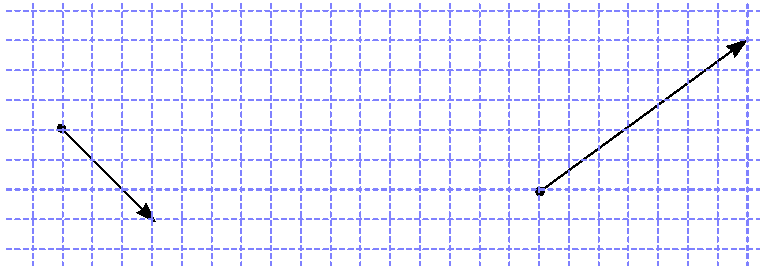
\includegraphics[width=0.65\textwidth]{2021-v2g-09-yl.pdf}
\end{center}



\hint

\solu
Valgusallika kiirusvektor ja kujutise kiirusvektor defineerivad kaks sirget, millest üks on teise kujutis. Need lõikuvad teadupärast läätse tasandil. Pikendades kiirusvektoreid lõikumiseni leiame nimetatud sirgete lõikepunkti $E$, mis asub läätsel. \pp3 \par
Valgusallikat ja selle kujutist ühendav sirge $AB$ peab läbima läätse keskpunkti. \pp1 \par
Sama peab kehtima sirge jaoks, mis ühendab valgusallika ja kujutise asukohti hästi lühikese ajavahemiku pärast. Üks võimalus ongi märkida valgusallika ja kujutise asukohad lühikese ajavahemiku $\Delta t$ pärast --- sellistes punktides $A'$ ja $B'$, kus nihkevektorid  $\vec{AA'}$ ja $\vec{BB'}$ on võrdelised vastavate kiirusvektoritega. \pp3 \par
Sellisel juhul saame leida läätse keskpunkti kui sirgete $AB$ ja $A'B'$ lõikepunkti. \pp2 \par
Probleem on selles, et niimoodi leitud asukoht on ebatäpne, sest kaks sirget lõikuvad väga väikese nurga all. Oluliselt täpsema tulemuse saame, kui paneme tähele, et projitseerides nihkevektorid $\vec{AA'}$ ja $\vec{BB'}$ sirge $AB$ ristsihile vektoriteks $\vec{AA''}$ ja $\vec{BB''}$ saame sirge $A''B''$, mis  lõpmatult lühikeste nihete puhul ühtib sirgega $A'B'$ ja mille lõikepunkt $O$ sirgega $AB$ püsib liikumatuna ka suurte nihete korral. Seetõttu võime punkti $O$ leidmiseks projitseerida kiirusvektorite lõpp-punktid sirge $AB$ ristsirgetele punktideks $C$ ja $D$. Sellisel juhul on punkt $O$ sirgete $AB$ ja $CD$ lõikepunktiks. \pp2 \par
Läätse tasandiks on sirge $OE$ ja läätse keskpunktiks punkt $O$ \pp1.
\begin{figure}[H]
  \centering
  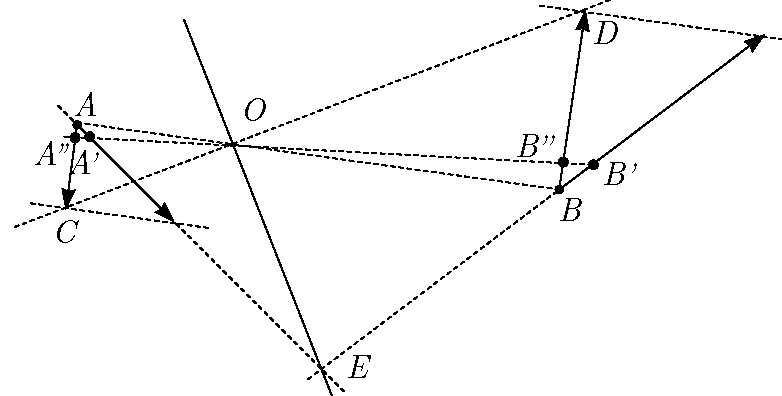
\includegraphics[width=0.69\textwidth]{2021-v2g-09-sol.pdf}
\end{figure}

\emph{Märkus:} \\
Väide, et punkt $A'$ kujutub punktiks $B'$ kehtib ainult siis, kui punktid $A'$ ja $B'$ paiknevad lõpmata lähedal vastavalt punkidele $A$ ja $B$. Valgusallika kiirusvektori otspunkt ei kujutu kujutise kiirusvektori otspunktiks. Kui punktvalgusallikas liigub ise konstantse kiirusega, siis ei saa sama väita tema kujutise kiiruse kohta. Alloleval joonisel on kujutatud siniste täppidega konstantse kiirusega liikuva valgusallika asukohad võrdsete ajavahemike tagant ning punaste täppidega vastavate siniste täppide kujutised. Jooniselt on näha, et punased täpid ei paikne võrdsete vahedega, järelikult kujutis ei liigu konstantse kiirusega.

\begin{figure}[H]
  \centering
  \begin{tikzpicture}[scale=0.3]
    \draw[{<[scale=1.6]}-{>[scale=1.6]}] (0.60294118, 10.20588235) -- (9.27941176, -11.44117647);
    \draw (-2.2745098 , -3.50980392) edge[dashed] (26.58823529,  8.05882353);
    \filldraw [blue]
    (0.0, 0.0) circle (3pt)
    (0.25, -0.25) circle (3pt)
    (0.5, -0.5) circle (3pt)
    (0.75, -0.75) circle (3pt)
    (1.0, -1.0) circle (3pt)
    (1.25, -1.25) circle (3pt)
    (1.5, -1.5) circle (3pt)
    ;
    \filldraw [red]
    (16.0, -2.0) circle (3pt)
    (16.65056497175141, -1.5353107344632768) circle (3pt)
    (17.470625798212005, -0.9495530012771394) circle (3pt)
    (18.5363436123348, -0.1883259911894275) circle (3pt)
    (19.977547495682206, 0.8411053540587212) circle (3pt)
    (22.035115303983222, 2.310796645702305) circle (3pt)
    (25.212, 4.58) circle (3pt)
    ;
  \end{tikzpicture}
\end{figure}
\probend